\documentclass{beamer}
%\documentclass[aspectratio=169]{beamer}
%
\mode<presentation>
{
  \usetheme{default}      
  \usecolortheme{default}
  \usefonttheme{default} 
  \setbeamertemplate{navigation symbols}{}
  \setbeamertemplate{caption}[numbered]
} 

\usepackage[english]{babel}
\usepackage[utf8x]{inputenc}
\usepackage{amsmath}
\usepackage{bm}
\usepackage{bbm}

\newcommand{\X}{\mathcal{X}}
\newcommand{\Y}{\mathcal{Y}}
\newcommand{\real}{\mathbb{R}}
\newcommand{\N}{\mathbb{N}}
\newcommand{\yhat}{\hat{y}}
\newcommand{\bxi}{\bm{x}^{(i)}}
\newcommand{\bx}{\bm{x}}
\newcommand{\xij}{x^{(i)}_j}
\newcommand{\yi}{y^{(i)}}
\newcommand{\yhati}{\hat{y}^{(i)}}
\newcommand{\norm}[1]{\left\lVert#1\right\rVert}
\newcommand{\1}[1]{\mathbbm{1}\left[#1\right]}

\title[Course presentation]{Machine learning from scratch}
\subtitle{Lecture 1: Mathematical background}
\author{Alexis Zubiolo\newline\texttt{alexis.zubiolo@gmail.com}}
\institute{Data Science Team Lead @ Adcash}
\date{January 26, 2017}

\begin{document}

\begin{frame}
  \titlepage
\end{frame}

\begin{frame}{Before we start}
IT STEP will be organizing a Tech night on \textbf{February 16th} (Thursday) from 7pm. I will (probably) be giving a talk. The course will most likely be postponed.
\end{frame}

\begin{frame}{Motivation, vocabulary and notations}
In \textbf{supervised learning} tasks, we are given a \textit{data set} of the form:
$$ D = \left\{ \left(\bxi, \yi\right), \bxi \in \X, \yi \in \Y, i \in \{1, \dots, n \}  \right\}$$
\pause
\begin{itemize}
	\item $n$ is the size of the data set (number of \textit{instances}/\textit{samples})
	\item In most applications:
	\begin{itemize}
		\item $\X = \real^d$ ($d$ is the \textit{dimensionality})
		\item $\Y = \real$ (\textit{regression}) or $\Y \subset \N$ (\textit{classification})
	\end{itemize}		
	\item $\bx \in \X$ is the \textit{feature vector} and $y \in \Y$ is the \textit{label}
\end{itemize}
\end{frame}

\begin{frame}{Motivation, vocabulary and notations}
Solving a \textbf{supervised learning problem} is finding (or \textit{learning}) a function (or \textit{hypothesis}) $h : \X \mapsto \Y$ such that for $(\bx, y)\in D$, $h(\bx)$ is a \textit{good} estimation  (or approximation) of $y$.
\pause
\vfill
We often write $h(\bx) = \yhat$ ($\yhat$ is the \textit{prediction} of $\bx$ by $h$).
\pause
\vfill
This raises \textbf{2 questions}:
\begin{itemize}
	\item How to define $h$?
	\item How to assess whether $\yhat$ is a good approximation of $y$?
\end{itemize}
\end{frame}

\begin{frame}{Hypothesis parametrization}
$h$ is often defined by a parameter vector $\theta$ and can be noted $h_\theta$. \pause Several ways to parametrize $h$ exist:
\begin{itemize}
	\item \textbf{Linear model}: $h(\bx) = \theta^T \bx$
	\item \textbf{Polynomial kernel} (degree $k$): $h(\bx) = \left(1 + \theta^T \bx\right)^k$
	\item Other kernels exist, more on this when we talk about duality
	\item With a \textbf{neural net}, more on this later as well
	\item \ldots
\end{itemize}
\vfill
\pause
How you define $h$ highly depends on the application, for example:
\begin{itemize}
	\item Sometimes a lot of data preprocessing has been made and a simple model (e.g. linear) would work well
	\item You might have \textbf{time/hardware constraints}: In this case going for a too complex model might be crippling
	\item For neural net, the architecture depends a lot on the type of data you have
\end{itemize}
\end{frame}


\begin{frame}{Linear Algebra concepts (1)}
Recall the regression example from the previous lecture:
\pause
\vfill
\begin{table}
\centering
\begin{tabular}{r|r|r}
living area (m$^2$) &  \textbf{\# bedrooms} & price (1000's BGN) \\\hline
50 & \textbf{1} & 30\\
76 & \textbf{2} & 48\\
26 & \textbf{1} & 12\\
102 & \textbf{3} & 90\\
\pause
61 & \textbf{2} & ?
\end{tabular}
\end{table}
\vfill
\pause
Illustration of the introduced notations:
\begin{itemize}
	\item $\X = \real^2$ ($d = 2$ dimensions: living area and  \# bedrooms)
	\item $\Y = \real$ (regression task)
	\item $\bx^{(1)} = \left[ 50, 1 \right]^T$ and $y^{(1)} = 30000$
\end{itemize}
\end{frame}

\begin{frame}{Linear algebra concepts (2)}
\begin{table}
\centering
\begin{tabular}{r|r|r}
living area (m$^2$) &  \textbf{\# bedrooms} & price (1000's BGN) \\\hline
50 & \textbf{1} & 30\\
76 & \textbf{2} & 48\\
26 & \textbf{1} & 12\\
102 & \textbf{3} & 90\\
\end{tabular}
\end{table}
\vfill
\pause
Using a \textbf{linear regression model} gives
\begin{equation*}
h_\theta(\bx) = \theta_0 + \theta_1 x_1 + \theta_2 x_2
\end{equation*}
Generalization to any dimensionality $d$:
\begin{equation*}
h(\bx) = \sum_{j = 0}^{d} \theta_j x_j = \theta^T \bx
\end{equation*}
Here, we set $\bx_0 = 1$ so that $\theta_0$ is included in $\theta$. $\theta^T \bx$ is called the dot product (or inner product) between $theta$ and $\bx$ and is sometimes noted $\langle {\theta, \bx} \rangle$.
\end{frame}

\begin{frame}{Ordinary least squares}
\begin{table}
\centering
\begin{tabular}{r|r|r}
living area (m$^2$) &  \textbf{\# bedrooms} & price (1000's BGN) \\\hline
50 & \textbf{1} & 30\\
76 & \textbf{2} & 48\\
26 & \textbf{1} & 12\\
102 & \textbf{3} & 90\\
\end{tabular}
\end{table}
\vfill
\begin{equation*}
h(\bx) = \sum_{j = 0}^{d} \theta_j x_j = \theta^T \bx
\end{equation*}
\pause
\vfill
Suppose we chose the following loss function:
\begin{equation*}
\ell \left( y, \yhat \right) = \dfrac{1}{2} \left( y - \yhat \right)^2
\end{equation*}
This leads to the following least squares \textit{cost function}:
\begin{equation*}
J(\theta) = \dfrac{1}{2} \sum_{i = 1}^{n} \left( h\left(\bxi\right) - \yi \right)^2
\end{equation*}
This problem the \textbf{ordinary least squares} (OLS) regression model.
\end{frame}

\begin{frame}{Least Mean Squares (LMS) update rule}
We want to minimize the following cost function:
\begin{equation*}
J(\theta) = \dfrac{1}{2} \sum_{i = 1}^{n} \left( h\left(\bxi\right) - \yi \right)^2
\end{equation*}
One way to do it is by using the \textbf{gradient descent} algorithm:
\begin{equation*}
\theta_j := \theta_j - \alpha \dfrac{\partial}{\partial \theta_j} J(\theta)
\end{equation*}
for all $j \in \{ 0, \dots, d\}$. $\alpha$ is called the \textbf{step size} or the \textbf{learning rate}. This update rule can be rewritten in a more compact way:
\begin{equation*}
\theta := \theta - \alpha \nabla J(\theta)
\end{equation*}
where $\nabla J(\theta)$ is the \textbf{gradient} of $J$ in $\theta$. We have, by definition:
\begin{equation*}
\nabla J(\theta) = \left[ \dfrac{\partial}{\partial \theta_1} J(\theta), \dots, \dfrac{\partial}{\partial \theta_d} J(\theta) \right]^T
\end{equation*}
\end{frame}

\begin{frame}{Least Mean Squares (LMS) update rule}
To apply the LMS update rule, we need to compute the gradient of $J$. Let's compute it for a single $(\bx, y)$ sample:
\begin{equation*}
\begin{split}
\dfrac{\partial}{\partial \theta_j} J(\theta) & = \dfrac{\partial}{\partial \theta_j} \dfrac{1}{2} \left( h\left(\bx\right) - y \right)^2 \\ 
 & = \text{?} \\
\end{split}
\end{equation*}
\textbf{Exercise}: Compute the gradient and find the update rule.
\end{frame}

\begin{frame}{Least Mean Squares (LMS) update rule}
Solution: 
\begin{equation*}
\begin{split}
\dfrac{\partial}{\partial \theta_j} J(\theta) & = \dfrac{\partial}{\partial \theta_j} \dfrac{1}{2} \left( h\left(\bx\right) - y \right)^2 \\ 
 & = 2 \dfrac{1}{2} \left( h\left(\bx\right) - y \right) \dfrac{\partial}{\partial \theta_j}\left( h\left(\bx\right) - y \right)\\
 & = \left( h\left(\bx\right) - y \right) \dfrac{\partial}{\partial \theta_j}\left( \sum_{k = 1}^{d} \theta_k x_k - y \right)\\
 & = \left( h\left(\bx\right) - y \right) x_j\\
\end{split}
\end{equation*}
\pause
\vfill
So the gradient descent update becomes
\begin{equation*}
\begin{split}
\theta_j &:= \theta_j - \alpha \dfrac{\partial}{\partial \theta_j} J(\theta) \\
 & := \theta_j + \alpha \left( y - h\left(\bx\right)\right) x_j
\end{split}
\end{equation*}
\end{frame}

\begin{frame}{LMS update rule interpretation}
LMS update rule for one sample:
\begin{equation*}
 \theta_j := \theta_j + \alpha \left( y - h\left(\bx\right)\right) x_j
\end{equation*}
\vfill
\pause
A few intuitive \textbf{interpretations}:
\begin{itemize}
	\item The magnitude of the step we make is proportional to $\alpha$
	\item The magnitude of the step we make is proportional to $ \left( y - h\left(\bx\right)\right)$, which is \textbf{the error} we make:
	\begin{itemize}
		\item If $h\left(\bx\right) \approx y$, then we won't move much
		\item Else, we will make a bigger step
	\end{itemize}
\end{itemize}
\vfill
\pause
Given this update rule, we can derive two different algorithms:
\begin{itemize}
	\item Batch gradient descent
	\item Stochastic gradient descent
\end{itemize}
\end{frame}

\begin{frame}{LMS update rule interpretation: batch updates}
LMS update rule for one sample:
\begin{equation*}
 \theta_j := \theta_j + \alpha \left( y - h\left(\bx\right)\right) x_j
\end{equation*}
\pause
\vfill
\textbf{Exercise}: What would be the batch gradient update rule?
\pause
\vfill
\textbf{Solution}: Repeat, until \textit{convergence}: For every $j \in \left\{ 1, \dots, d\right\}$:
\begin{equation*}
\theta_j := \theta_j + \alpha \sum_{i = 1}^n \left(\yi - h\left(x^{(i)}_j\right)\right) x^{(i)}_j
\end{equation*}

\end{frame}

\begin{frame}{LMS update rule interpretation: Stochastic updates}

LMS update rule for one sample:
\begin{equation*}
 \theta_j := \theta_j + \alpha \left( y - h\left(\bx\right)\right) x_j
\end{equation*}
\pause
\vfill
\textbf{Exercise}: What would be the batch stochastic update rule?
\pause
\vfill
\textbf{Solution}: Repeat, until \textit{convergence}: For $i \in \left\{1, \dots, n \right\}$, for every $j \in \left\{ 1, \dots, d\right\}$:
\begin{equation*}
\theta_j := \theta_j + \alpha \sum_{i = 1}^n \left(\yi - h\left(x^{(i)}_j\right)\right) x^{(i)}_j
\end{equation*}
Here, $\theta$ is updated everytime we read a sample!
\end{frame}

\begin{frame}{Optimization convergence}
The batch and stochastic gradient descents we discussed iterate until convergence. How do we know whether the algorithm has converged or now?
\vfill
\pause
We usually check the difference between two successive values of $J(\theta)$.
\end{frame}

\begin{frame}{Standard loss functions}
0-1 loss:
$$ \ell \left( \hat{y}, y \right) = \1{\hat{y} = y}$$
\vfill
\pause
Squared loss:
$$ \ell \left( \hat{y}, y \right) = \left( \hat{y} - y\right)^2$$
\vfill
\pause
Hinge loss:
$$ \ell \left( \hat{y}, y \right) = \max\left(0, 1 - \hat{y} y\right)$$
\vfill
\pause
Squared hinge loss:
$$ \ell \left( \hat{y}, y \right) = \max\left(0, 1 - \hat{y} y\right)^2 $$
\vfill
\pause
Log-loss:
$$ \ell \left( \hat{y}, y \right) = \log \left( 1 + \exp ( - \hat{y}y )\right) $$
\end{frame}

\begin{frame}{Loss functions}
\begin{figure}
\centering
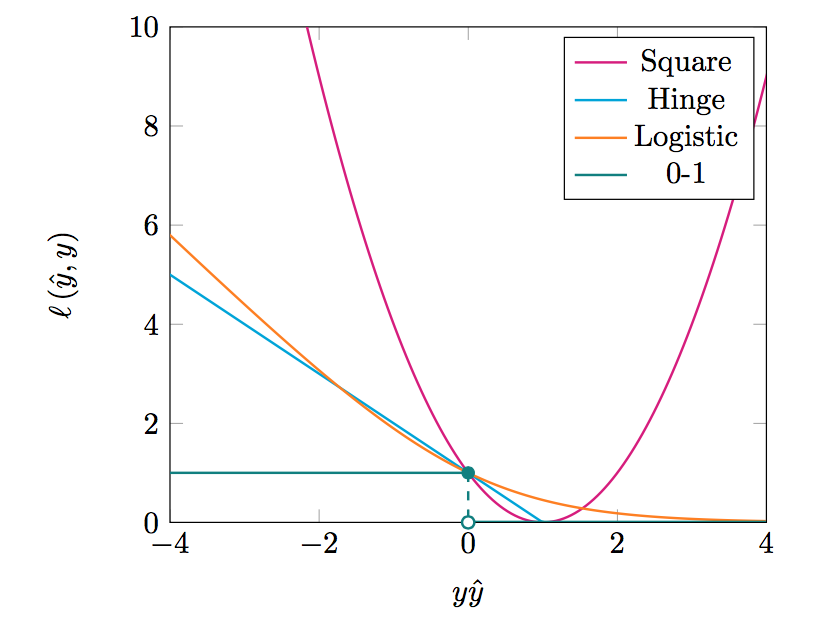
\includegraphics[width=\linewidth]{images/losses.png}
\end{figure}
\end{frame}

\begin{frame}{Conclusion}
We have seen the motivation and the formalization of a supervised learning problem with a basic example.
\vfill
\pause
Next week, there will be some implementation tasks to do. You can work on the machines at IT STEP, but feel free to bring your laptop if you prefer.
\vfill
\pause
Also, we still have to see more general concepts about optimization, statistical interpretations, regularization.
\end{frame}

\begin{frame}
\vfill
\centering
\begin{huge}
\huge{Thank you! Questions?}
\vfill
\texttt{alexis.zubiolo@gmail.com}
\end{huge}
\vfill
\begin{Large}
\texttt{https://github.com/azubiolo/itstep}
\end{Large}
\vfill
\end{frame}

\end{document}
